\paragraph{Мейн}
В этой задаче мы снова имеем дело с модулем ядра, который не запускается напрямую как исполняемый файл, но доступен для анализа через вывод команды \texttt{strings} и в ghidra.

\paragraph{Описание}
\begin{enumerate}
    \item Попытка запуска файла с правами суперпользователя:
    \begin{verbatim}
    m@hp:~/Downloads/1$ sudo ./task_3
    [sudo] password for m:
    sudo: ./task_3: command not found
    \end{verbatim}
    Вывод: команда не найдена. Скорее всего, файл не является исполняемым бинарником, а модулем ядра.

    \item Просмотр строк в файле через \texttt{strings}:
    \begin{verbatim}
    m@hp:~/Downloads/1$ strings task_3
    Linux
    Linux
    AUATI
    A]A^]1
    flag
    itmo
    6[*] Bye - bye !
    1reading...
    1[*] Error assigning Major Number!
    1[*] Failed to register device class
    1[*] Failed to create the device
    G'g/|
    W[0sd
    q-fn
    rEdWcNDyavDSNOdKOC95iTEP8bioF3IPmAKUXx
    license=GPL
    description=find the flag
    srcversion=0765CAD67B0F0DF80A62408
    depends=
    retpoline=Y
    name=task_8
    vermagic=6.2.0-34-generic SMP preempt mod_unload modversions
    __register_chrdev
    __class_create
    device_create
    __x86_return_thunk
    _printk
    class_destroy
    __unregister_chrdev
    device_destroy
    class_unregister
    vmalloc
    __check_object_size
    _copy_to_user
    __copy_overflow
    __fentry__
    module_layout
    task_8
    GCC: (Ubuntu 11.4.0-1ubuntu1~22.04) 11.4.0
    GCC: (Ubuntu 11.4.0-1ubuntu1~22.04) 11.4.0
    __UNIQUE_ID_srcversion193
    __UNIQUE_ID_depends192
    ____versions
    __UNIQUE_ID_retpoline191
    __UNIQUE_ID_name190
    __UNIQUE_ID_vermagic189
    _note_10
    _note_9
    intro_init
    fops
    __key.11
    my_class
    intro_exit
    __UNIQUE_ID___addressable_cleanup_module241
    __UNIQUE_ID___addressable_init_module240
    __UNIQUE_ID_license239
    __UNIQUE_ID_description238
    __pfx_intro_read
    __check_object_size
    __class_create
    __this_module
    class_destroy
    crypted
    __fentry__
    _printk
    __copy_overflow
    __pfx_init_module
    major
    device_create
    class_unregister
    __pfx_cleanup_module
    __x86_return_thunk
    _copy_to_user
    __register_chrdev
    device_destroy
    vmalloc
    __unregister_chrdev
    .symtab
    .strtab
    .shstrtab
    .note.gnu.build-id
    .note.Linux
    .rela.text
    .rela.init.text
    .rela.exit.text
    .rodata.str1.1
    .rodata.str1.8
    .rela__mcount_loc
    .rodata
    .modinfo
    .rela.return_sites
    .rela.call_sites
    __versions
    .rela__patchable_function_entries
    .rela.data
    .rela.exit.data
    .rela.init.data
    .rela.gnu.linkonce.this_module
    .bss
    .comment
    .note.GNU-stack
    \end{verbatim}

    \item Анализ строк:
    \begin{itemize}
        \item В выводе присутствует строка \texttt{flag}, но не полный флаг.
        \item Присутствует строка, напоминающая шифрованные данные:
        \begin{verbatim}
        rEdWcNDyavDSNOdKOC95iTEP8bioF3IPmAKUXx
        \end{verbatim}
        \item Также указано описание:
        \begin{verbatim}
        description=find the flag
        \end{verbatim}
    \end{itemize}
    Предполагаю, что флаг зашифрован и хранится в строке \texttt{crypted}.

    \item После этого, в ghidra, через дизассемблированную фунцию \_\_pfx\_init\_module я нашел функцию \_\_pfx\_intro\_read:

    \begin{verbatim}
    undefined1 [16] __pfx_intro_read(undefined8 param_1, undefined8 param_2, ulong param_3) {
  long lVar1;
  byte bVar2;
  long lVar3;
  byte bVar4;

  _printk(&DAT_001006b3);
  lVar1 = vmalloc(0x27);
  bVar2 = 0x14;
  bVar4 = 0x72;
  lVar3 = 0;

  while (true) {
    *(byte *)(lVar1 + lVar3) = bVar2 ^ bVar4;
    if (lVar3 + 1 == 0x26) break;
    bVar4 = "rEdWcNDyavDSNOdKOC95iTEP8bioF3IPmAKUXx"[lVar3 + 1];
    bVar2 = crypted[lVar3 + 1];
    lVar3 = lVar3 + 1;
  }
  *(undefined1 *)(lVar1 + 0x26) = 0;

  if (param_3 < 0x28) {
    __check_object_size(lVar1, param_3, 1);
    _copy_to_user(param_2, lVar1, param_3);
  } else {
    __copy_overflow(0x27, param_3);
  }
  return ZEXT816(0);
}
    \end{verbatim}

    \item Размышления: Эта функция - дешифратор. Мы можем заметить тут наш зажифрованный флаг, который обнаружили ранее, а также массив \texttt{crypted}. Эта функция посимвольно делает XOR с элементами массива и расшифровывает флаг.

    \item Массив \texttt{crypted} я нашел в сегменте .rodata. Теперь можно составить несложный питон скрипт для дешифровки флага:
    \begin{verbatim}
        crypted = [
    0x14, 0x29, 0x05, 0x30, 0x18, 0x7d, 0x70, 0x4a, 0x03, 0x47,
    0x27, 0x67, 0x2f, 0x7c, 0x01, 0x2a, 0x78, 0x71, 0x08, 0x57,
    0x5b, 0x30, 0x73, 0x64, 0x08, 0x04, 0x0a, 0x57, 0x71, 0x03,
    0x79, 0x34, 0x0f, 0x71, 0x2d, 0x66, 0x6e, 0x05
]

flag = "rEdWcNDyavDSNOdKOC95iTEP8bioF3IPmAKUXx"

decrypted = ''.join(chr(c ^ ord(f)) for c, f in zip(crypted, flag))

print(f"Decrypted flag: {decrypted}")

    \end{verbatim}
    \item После дешифровки мы получаем наш флаг - flag\{343b1c4a3ea721b2d640fc8700db0f36\}
\end{enumerate}

\vspace{0.5cm}

\noindent

\paragraph{Оссобенности}
\begin{itemize}
    \item Файл \texttt{task\_3} — это модуль ядра Linux.
    \item Флаг, зашифрован в строке:
    \begin{verbatim}
    rEdWcNDyavDSNOdKOC95iTEP8bioF3IPmAKUXx
    \end{verbatim}
    \item Метод шифрования - XOR
    \item После шифрования искомый флаг - flag\{343b1c4a3ea721b2d640fc8700db0f36\}
    \item В выводе присутсвует \("\)depends= \ldotsname=task\_8\ldots\("\), возможно этот файл содержит выводы для 8го задания
\end{itemize}

\paragraph{Тестовый запуски}
Оставлю тут вывод питоновского скрипта

\paragraph{}
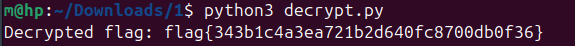
\includegraphics[width=1\linewidth]{static/solution_task_3}
